\subsection{Node}
\begin{center}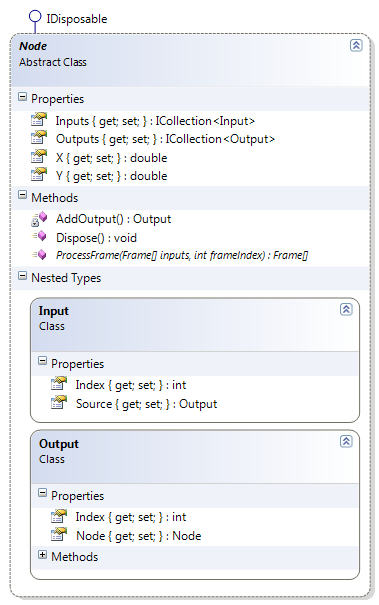
\includegraphics[scale=0.7]{YuvKA.Pipeline/node.png} \\
Die Basisklasse \name{Node} stellt die Attribute und Methoden zur Verfügung, welche von allen Knoten (seien dies Eingabe-, Ausgabe- oder Manipulationsknoten) benötigt werden. Dies umfasst die \name{ProcessFrame}-Methode, welche die tatsächliche Bearbeitung der \name{Frame}s darstellt, als auch alle Informationen bezüglich der Verbindungen zwischen verschiedenen Knoten, welche in den inneren Klassen \name{Input} und \name{Output} gestellt sind.
\end{center}

\subsubsection{YuvKA.Pipeline.Node}

\begin{verbatim}
[InheritedExport]
[DataContract]
public abstract class Node : IDisposable
\end{verbatim}

\paragraph{Beschreibung}~\\
Die Klasse \name{Node} stellt die gemeinsame Struktur aller Knoten zur Verfügung. Die allgemeine Arbeitsweise eines solchen Knotens besteht darin, dass er nach seiner Konstruktion und dem Verbinden seiner Eingänge durch einen Aufruf der Funktion \name{Processframe} zur Verarbeitung der gegebenen \name{Frame}s ab dem gegebenen Index gebracht wird.

\paragraph{Typmember}
\begin{itemize}

\property{X}
	\begin{verbatim}
	[Browsable(false)]
	[DataMember]
	public double X { get; set; }
	\end{verbatim}
	%<Membererklärung>
	==Hier bitte gute Rechtfertigung wieso ein Knoten seine Position wissen muss.==

%[etc.]

\method{ProcessFrame}
	\begin{verbatim}
	public abstract Frame[] ProcessFrame(Frame[] inputs, int tick);
	\end{verbatim}
	Verarbeitet die gegebenen \name{Frame}s entsprechend des internen Algorithmus' und gibt ein Array von \name{Frame}s als Resultat zurück. Der Parameter \name{inputs} ist hierbei direkt als die Daten, welche an den Eingängen des Knotens anliegen, zu interpretieren. Dementsprechend entspricht der Rückgabewert den Daten, welche an den Ausgängen des Knotens durchgereicht werden.

%[etc.]

\end{itemize}

%\subsubsection{<weitere Klasse im gleichen Format...>}
%Beschreibung, Member und Methoden, etc.

